\part{Adjarian's endmatter}
\chapter{Placenames and maps }

\translatorHD{This chapter is written by the translator (me). The content is based on the final pages of  Adjarian's book, where he provides  a list of placenames and a map.}

\section{List of placenames from Adjarian's endmatter}
In the original document, Adjarian has a chapter where he lists all the place-names that had Armenian populations. For each location, he likewise gave the page number that mentioned this location.  This chapter was on page   294 and it can translated as ``\textit{Alphabetical list of Armenian residences and described provinces}''. He states that ``\textit{in total, there is a sample of 102 provincial vernaculars}''. 

In my translation, I list the Armenian names that Adjarian used and their original page numbers. The parenthesis mark text samples. I keep the original alphabetical order, based on the Armenian word.

I likewise provide other common Armenian names for these locations (usually this other word is just the Armenian name with reformed spelling). I provide  the corresponding Romanized or English name. In general, the Romanized name is based on the most common name that is used in Latin-script sources, such as English Wikipedia. When multiple Romanizations are attested, we list all of them. We use the Romanization that is the most common in English, most commonly used by Armenians, or most closely resembles Adjarian's original Armenian name.

In some cases, I couldn't find the modern name or location of a placename. I give a hypothetical Romanization  with a question mark. 

In some cases, Adjarian provides a page number as an example of some place name, but that page doesn't actually have that place names. I did not  catalog such errors. 

I use archaic names such as Birmania instead of Myanmar, so that the translation does not seem anachronistic. 


\begin{center}
\begin{longtable}{|p{3.cm}|p{3cm}|p{3cm}|p{2cm}|p{3cm}|}
\caption{Adjarian's  list of Armenian residences and described provinces} \label{tab:long} \\ \hline
\hline Armenian term & Other Armenian  & Romanization   & Other   & Page \\ 
used by Adjarian  & terms&   that we use&romanizations & 
\\ \hline\hline
Ագուլիս & & 
{Agulis}   &Əylis &\ref{page:1}, \ref{page:2}, \ref{page:3}, \ref{page:4}, \ref{page:13}, \ref{page:36}, \ref{page:40}, \ref{page:89}, \ref{page:92}-100, (\ref{page:101}-2), \ref{page:104}\\ \hline
Ադամխան&  Վարդաձոր & 
{Adamxan} & Vardadzor
&\ref{page:116}, \ref{page:118}, (\ref{page:134})\\ \hline
Ադլեր&Ադլէր & 
{Adler}& &\ref{page:184}\\ \hline
Ադրիանուպօլիս&Ադրիանուպոլիս, Էդիրն
& {Adrianopolis}  & Adrianople,  Hadrianopolis, Edirne &\ref{page:29}, \ref{page:31}, \ref{page:258}\\ \hline
Ազով& &
{Azov}& &\ref{page:26}\\ \hline
Աթէնք& Աթենք&
{Athens}& &\ref{page:29}\\ \hline
Ալաշկերտ& &
{Alashkert}& Eleşkirt&\ref{page:10}, \ref{page:116}-7, \ref{page:121}, (\ref{page:125}), \ref{page:133}\\ \hline
Ալէքսանդրապոլ&Ալեքսանդրապոլ,  Ալէքսանդրապօլ,  Գյումրի
&{Alexandropol} & Gyumri&\ref{page:34}, \ref{page:104}, \ref{page:107}, \ref{page:111}, \ref{page:116}\\ \hline
Ալէքսանդրէտ&Ալեքսանդրետ, Ալեքսանդրետտա &
{Alexandretta}& İskenderun&\ref{page:199}\\ \hline
Ալիլու& 
&{Alilu}& &\ref{page:288}\\ \hline
Ալիկրըխ&Աստղաձոր &
{Alikrykh}&Astghadzor &\ref{page:116}, \ref{page:118}, (\ref{page:137})\\ \hline
Ալիղուլի& Հարթաշեն
& {Alighuli}& Hartashen&\ref{page:288}\\ \hline
Ալուշտա& &
{Alushta}& &\ref{page:26}\\ \hline
Ալուչալու&    Արծվանիստ 
&{Aluchalu} &Artsvanist &\ref{page:116}, \ref{page:118}, \ref{page:139}\\ \hline
Ախալցխա& 
&Akhaltskha   &Akhaltsikhe &\ref{page:2}, \ref{page:34}, \ref{page:104}, \ref{page:107}, \ref{page:111}\\ \hline
Ախալքալաք&Ախալքալաքի &  Akhalkalak 
& {Akhalkalaki}&\ref{page:31}, \ref{page:32}, \ref{page:34}, \ref{page:104}, \ref{page:111}, (\ref{page:113}), \ref{page:116}\\ \hline
Ածպտեր& Ազբդեր, Էզիդեր& 
{Adzbder} &Akıncılar, Ezbider &\ref{page:174}\\ \hline
Ակն& &
{Akn}&Kemaliye &\ref{page:29}, \ref{page:103}, \ref{page:222}-3, (\ref{page:224}), \ref{page:260}\\ \hline
Աղբակ& & 
{Aghbak}& &\ref{page:140}\\ \hline
Աղդաշ& & 
{Agdash}& &\ref{page:26}\\ \hline
Աղէքսանդրիա& Աղեքսանտրիա
&{Alexandria}& &\ref{page:28}\\ \hline
Աղուանք& Աղվանքx
& {Aghvank}&Caucasian Albania &\ref{page:25}\\ \hline
Աղստաֆա& Աղստև
& {Agstafa}& &\ref{page:61}\\ \hline
Ամասիա& & 
{Amasia}& &\ref{page:29}, \ref{page:232}, \ref{page:234}\\ \hline
Ամերիկա see Մ. Նահանգ.& &America, see the United States & &\\ \hline
Այթօս&Այթոս & 
{Aytos}& Aitos&\ref{page:29}, \ref{page:31}\\ \hline
Այնթապ& &
Ayntap& &\ref{page:28}, \ref{page:30}\\ \hline
Այտըն& Այդըն 
&{Aydın} & &\ref{page:29}, \ref{page:33}, \ref{page:293}\\ \hline
Անափա & &Anapa & & \ref{page:25} \\\hline 
Անգեղակոթ &   &Angeghakot & & \ref{page:288} \\ \hline 
Անգլիա & &England & & \ref{page:29}, \ref{page:33}, \ref{page:293} \\ \hline 
Անդիժան& & 
{Andijan}& &\ref{page:26}\\ \hline
Անտիոք or Անթաքիա& & 
Antioch& Antakya &\ref{page:28}, \ref{page:199}, \ref{page:200}, (\ref{page:210}), \ref{page:212}\\ \hline
Աշտարակ& & 
{Ashtarak}& &\ref{page:105}\\ \hline
Ապարան& & 
{Aparan}& &(\ref{page:116}-7, \ref{page:121}, (\ref{page:126})\\ \hline
Ապկիօն& &
{Abgion?}\footnote{I couldn't track down}& &(\ref{page:194}, \ref{page:185}\\ \hline
Առըս& & 
{Arəs?}\footnote{I couldn't track down.}&&\ref{page:26}\\ \hline
Առնջկոյս&Առնջկուս
& Arinjkus& Kavuştuk       &(\ref{page:132})\\ \hline
Ասլանբէկ& Ասլանբեկ, Ասլանբէգ& 
{Aslanbeg}&Arslanbey, Aslanbey &\ref{page:3}, \ref{page:12}-13, \ref{page:106}, \ref{page:175}, \ref{page:241}-4, (\ref{page:244}-5)\\ \hline
Ասխաբադ& & 
{Ashgabat}& &\ref{page:26}\\ \hline
Ասորեստան& & 
Assyria& modern Iraq&\ref{page:27}, \ref{page:33}\\ \hline
Ասորիք տես Սիւրիա& &  historical Syria, see Syria&   &\\ \hline
Աստապատ& & 
{Astabad}& &\ref{page:37}, \ref{page:45}-47, (\ref{page:48})\\ \hline
Աստրախան& Աժտէրխան& 
{Astrakhan}& &\ref{page:26}, \ref{page:30}, \ref{page:36}, \ref{page:82}-84, (\ref{page:84}-86), \ref{page:89}\\ \hline
Ատանա& Ադանա& &
Adana&\ref{page:28}\\ \hline
Ատափազար& & 
Adapazar  &Adapazarı &\ref{page:13}, \ref{page:29}, \ref{page:241}, (\ref{page:246})\\ \hline
Ատիեաման& Ադըյաման& 
{Adıyaman}& &\ref{page:29}, \ref{page:196}, (\ref{page:198})\\ \hline
Ատրպատական& & 
{Atropatene}& Iranian Azerbaijan&\ref{page:27}, \ref{page:37}, \ref{page:70}\\ \hline
Արաբկիր& &
Arapgir &Arabkir &\ref{page:3}, \ref{page:4}, \ref{page:29}, \ref{page:103}, \ref{page:196}, \ref{page:215}-6, (\ref{page:217}), \ref{page:222}-3\\ \hline
Արամօ& Արամո, Արամոյ
&Aramo & &\ref{page:28}, \ref{page:212}-3, (\ref{page:213}-4)\\ \hline
Արդուին&Արդվին, Արթվին  &Artvin&
 &\ref{page:19}, \ref{page:25}, \ref{page:34}, \ref{page:280}, \ref{page:291}-2, (\ref{page:292})\\ \hline
Արեւելեան Ռումէլի&Ռումելիա
& {Eastern Rumelia} & &(\ref{page:31}-32\\ \hline
Արթղ& &
{Artəgh?}\footnote{I couldn't track down.}& &\ref{page:26}\\ \hline
Արծափ& &  {Ardzap}& Sağlıksuyu&\ref{page:138}\\ \hline
Արծկէ& Արծկե
& {Artske} &Adilcevaz &\ref{page:117}, \ref{page:118}, \ref{page:121}, (\ref{page:132})\\ \hline
Արղնի& Արկնի  
&{Arghni} & Ergani&\ref{page:159}\\ \hline
Արճէշ& Արճեշ, Ականց& 
{Arjesh}& Erciş&(\ref{page:116}-8, \ref{page:121}, (\ref{page:131}), \ref{page:139}\\ \hline
Արմաւիր& Արմավիր&
Armavir& &\ref{page:26}, \ref{page:33}\\ \hline
Արմեանսկ&Արմյանսկ
&Armiansk & &\ref{page:26}\\ \hline
Արտահան&Արդահան & 
{Ardahan}&&\ref{page:291}\\ \hline
Արտանուշ&Արտանուջ 
& {Ardanuç}& Artanuj&\ref{page:25}, \ref{page:291}\\ \hline
Արտապիլ& Արդաբիլ&
{Ardabil}& &\ref{page:28}\\ \hline
Աւդալաղալու&Աւտալաղալու, Ավդալաղալու, Վաղաշեն &
{Avdalaghalu}&Vaghashen &\ref{page:116}, \ref{page:118}, (\ref{page:137})\\ \hline
Աւստրօ-Հունգարիա&Ավստրո-Հունգարիա
&Austro-Hungary &Austria-Hungary &\ref{page:10}, \ref{page:19}, \ref{page:27}, \ref{page:103}, \ref{page:270}-2, (\ref{page:273}-9)\\ \hline
Աքքերման&Աքքիրման,  Բելգորոդ-Դնեստրովսկի&
{Akkerman}& Bilhorod-Dnistrovskyi&\ref{page:27}, \ref{page:31}\\ \hline
Աֆիօն-Գարահիսար&Աֆիոն-Կարահիսար
& Afyonkarahisar& &\ref{page:29}\\ \hline
Բաբերդ& Բայբերդ&
{Baberd} &Bayburt &\ref{page:13}, \ref{page:111}-2\\ \hline
Բագու& &
Baku& &\ref{page:13}, \ref{page:25}, \ref{page:61}, \ref{page:76}\\ \hline
Բազարքէօյ&  
&Pazarköy& &\ref{page:241}\\ \hline
Բաթում& Բաթումի& 
{Batumi}& &\ref{page:13}, \ref{page:25}, \ref{page:32}, \ref{page:34}, \ref{page:178}, \ref{page:291}\\ \hline
Բալակ& & 
Balak & &\ref{page:288}\\ \hline
Բալաշով& &  {Balashov}& &\ref{page:26}\\ \hline
Բալու& &
{Palu}& Balu&\ref{page:167}, \ref{page:168}\\ \hline
Բաղէշ& Բաղեշ, Պիթլիս,  Բիթլիս & {Paghesh}&Baghesh, Bitlis &\ref{page:33}, \ref{page:116}-8, \ref{page:121}, (\ref{page:131})\\ \hline
Բաղչէսարայ& Բաղչեսարայ, Բաղչէսէրայ&{Bakhchisaray} & Baghchesaray, Eski Yurt&\ref{page:26}, \ref{page:263}\\ \hline
Բաշքէնդ &Բաշքենդ, Բաշգենդ &{Bashkent} & &\ref{page:37}\\ \hline
Բասարգեչար& Վարդենիս &
{Basargechar}&Vardenis &\ref{page:140}, \ref{page:145}-6, (\ref{page:152}-4)\\ \hline
Բասեն& &Basean & 
{Phasiane},     Pasinler &\ref{page:111}, (\ref{page:114})\\ \hline
Բատալբաշու& &
{Batalbashu?}\footnote{I couldn't track down this town. }& &\ref{page:26}\\ \hline
Բաւրա& Բավրա
& {Bavra}& &\ref{page:31}\\ \hline
Բաֆոս&Պաֆոս
& {Paphos}& Bafos&\ref{page:28}\\ \hline
Բեթղեհեմ&Բեթղեհէմ &
Bethlehem& &\ref{page:27}\\ \hline
Բելցի& Բէլցի&
{Balti}& Beltsi&\ref{page:27}, \ref{page:31}\\ \hline
Բենդեր& Բէնդէր&
{Bender}& &\ref{page:27}, \ref{page:31}\\ \hline
Բեշթա& Բէթա& 
{Beshta?} \footnote{I couldn't track down.}& &\ref{page:27}\\ \hline
Բեսարաբիա&  &Bessarabia & &\ref{page:27}, \ref{page:31}, \ref{page:32}\\ \hline
Բերդեանսկ&Բերդյանսկ &
{Berdiansk}&Berdyansk &\ref{page:26}\\ \hline
Բթեշտ&Պիտեշտ 
&{Pitești}  &    &\ref{page:27}\\ \hline
Բլօէշտի& Պլոեշտի
&{Ploiești}& &\ref{page:27}\\ \hline
Բոլնիս-Խաչէն& Բոլնիս-Խաչեն
& Bolnis-Khachini& Bolnisi&\ref{page:61}, \ref{page:62}\\ \hline
Բորչալու& 
&{Borchaly} & &\ref{page:37}, \ref{page:47}\\ \hline
Բուխարա& &
{Bukhara}& &\ref{page:26}\\ \hline
Բուշիր& & 
{Bushehr}&Bushire &\ref{page:87}\\ \hline
Բրգնիկ& &
{Pirknik}& Dörteylül& \ref{page:225}, \ref{page:227}\\ \hline
Գահիրէ& Կահիրե
&Cairo & &\ref{page:28}\\ \hline
Գանձակ& Ելիզավետպոլ& 
Gandzak & Ganja, Elisabethpol&\ref{page:61}, \ref{page:52}, \ref{page:70}, \ref{page:72}, (\ref{page:74})\\ \hline
Գանձակ գիւղ& &
Gandzak village& &\ref{page:139}\\ \hline
Գանտիա& Հերակլիոն& 
{Kandiye}&Heraklion  & \ref{page:29}\\ \hline
Գասապա& & 
{Kasaba}& Turgutlu&\ref{page:239}\\ \hline
Գասթամունի& Քասթամոնու, Քասթամունի&
  Kastamonu& Kastamoni& \ref{page:29}, \ref{page:30}\\ \hline
Գետակբուլաղ&Կարճաղբյուր 
& {Gedakbulag}&Karchaghbyur &\ref{page:116}, \ref{page:118}, (\ref{page:139})\\ \hline
Գերմանիա& & 
Germany& &\ref{page:30}\\ \hline
Գեօլ&Գյոլ
&{Gölköy} & &\ref{page:116}, \ref{page:118}, (\ref{page:135})\\ \hline
Գեօքչայ&Գյոքչայ
&{Geokchay} &Goychay &\ref{page:25}\\ \hline
Գըրգաղաճ& 
&Kırkağaç & &\ref{page:239}\\ \hline
Գիրգորէս&  
&{Girgores}?\footnote{I oculdn't track down.} & &\ref{page:232}\\ \hline
Գոլոդնայա-Ստէպ& Սովյալ տափաստան& 
Golodnaya Steppe& Mirzachoʻl&\ref{page:26}\\ \hline
Գոնիա& Քոնիա& 
{Konya}& &\ref{page:29}\\ \hline
Գորի& & 
{Gori}& &\ref{page:25}, \ref{page:32}\\ \hline
Գութի& &
{Guti?}\footnote{I couldn't track down.}&  &\ref{page:27}, \ref{page:33}\\ \hline
Գուլասոր& &
 Gulasor?\footnote{I couldn't track down.}& &\ref{page:138}\\ \hline
Գրիգորուպօլիս&Գրիգորիոպոլիս
& {Grigoriopol}& &\ref{page:27}, \ref{page:31}\\ \hline
Դալիղարդաշ&Սարուխան
& {Dalikardash}& Sarukhan&\ref{page:37}\\ \hline
Դաղստան& & 
{Dagestan}& &\ref{page:26}\\ \hline
Դամասկոս& &
Damascus& &\ref{page:28}, \ref{page:33}\\ \hline
Դաշտ& & 
{Dasht}& &\ref{page:92}\\ \hline
Դարբանդ& Դերբենդ?&
{Darband}&Derbent?\footnote{There are many locations in the area so it's difficult to know which exact city he meant. What's certain is that this city or village must have been in Caucasian Albania. \url{https://en.wikipedia.org/wiki/Darband}}, Karmrakar? &\ref{page:26}, \ref{page:61}, \ref{page:62}\\ \hline
Դիզակ& Հադրութ& 
Dizak &Hadrut &\ref{page:68}\\ \hline
Դիլիջան& &
Dilijan& &\ref{page:13}, \ref{page:61}\\ \hline
Դնեպր&Դնիպրո, Դնեբր & 
{Dnipro}& &\ref{page:26}, \ref{page:263}\\ \hline
Դուլակ& &
{Dulak}& &\ref{page:26}\\ \hline
Դուշէթ& Դուշեթ
&{Dusheti} & &\ref{page:25}\\ \hline
Դուրովկա& 
&{Durovka?}\footnote{I couldn't track this down} & &\ref{page:26}\\ \hline
Եալթա& Յալտա&{Yalta} 
& &\ref{page:26}, \ref{page:178}, \ref{page:263}\\ \hline
Եալովա& Յալովա
&{Yalova} & &\ref{page:241}\\ \hline
Եամպոլի& Եամպօլի, Յամպոլի&
{Yampil}&Yampol &\ref{page:29}, \ref{page:31}\\ \hline
Եաշ&Յաշ &Iași & &\ref{page:27}\\ \hline
Եաֆա&Յաֆֆա & Jaffa& &\ref{page:28}\\ \hline
Եգիպտոս& & Egypt& &\ref{page:28}, \ref{page:34}, \ref{page:293}\\ \hline
Եդեսիա& & Edessa&Edesia &\ref{page:29}, \ref{page:159}, (\ref{page:166})\\ \hline
Եթովպիա& &Ethiopia & &\ref{page:28}\\ \hline
Եկատերինոդար& &Yekaterinodar & &\ref{page:26}, \ref{page:263}\\ \hline
Եկատերինոսլավ& Եկատերինասլաւ &Yekaterinoslav & Dnipro&\ref{page:26}, \ref{page:263}\\ \hline
Եղիսաբեթուպօլիս &Դումբրըվեն &Elisabethopolis  &Dumbrăveni &\ref{page:27}, \ref{page:33}\\ \hline
Եյսկ& & Yeysk& &\ref{page:26}\\ \hline
Երանոս& &Yeranos & &\ref{page:116}, \ref{page:118}, (\ref{page:133})\\ \hline
Երեւան&Երևան &Yerevan &Erevan &\ref{page:4}, \ref{page:13}, \ref{page:36}-52, (\ref{page:47}), \ref{page:54}, \ref{page:55}, \ref{page:61}, \ref{page:62}, \ref{page:66}, \ref{page:70}, \ref{page:82}-3, \ref{page:88}-9, \ref{page:92}, \ref{page:95}-6, \ref{page:104}, \ref{page:106}, \ref{page:116}\\ \hline
Երզնկա&Էրզինկեան & Yerznka&Erzincan     &(\ref{page:103}-4), \ref{page:167}-174, (\ref{page:171}), \ref{page:197}, \ref{page:225}\\ \hline
Երուսաղէմ& Երուսաղեմ& Jerusalem& &\ref{page:28}\\ \hline
Եւդոկիա  &Եվդոկիա,  Թօքատ, Թօքաթ, Թոքաթ& Evdokia & Tokat &\ref{page:3}, \ref{page:29}, \ref{page:31}, \ref{page:103}, \ref{page:174}, \ref{page:178}, \ref{page:232}-4, \ref{page:239}, (\ref{page:234}-7), \ref{page:243}\\ \hline
Եւպատորիա& Եվպատորիա&Yevpatoriya & Eupatoria&\ref{page:26}, \ref{page:263}\\ \hline
Եւրոպական Թուրքիա& &European Turkey & &\ref{page:29}, \ref{page:31}, \ref{page:258}\\ \hline
Եօզղատ&Եոզղատ,   Յոզղատ  &Yozgat & &\ref{page:29}, \ref{page:32}, \ref{page:215}\\ \hline
Եօզղատ գիւղերը& &Yozgat villages & &\ref{page:31}, \ref{page:205}, \ref{page:215}\\ \hline
Զաղալու& Ախպրաձոր, Ծովակ& Zaghalu&Akhpradzor, Tsovak &\ref{page:116}, \ref{page:118}, (\ref{page:139})\\ \hline
Զանգեզուր& Զանկեզուր&Zangezur & &(\ref{page:75}), \ref{page:288}\\ \hline
Զառա& &Zara & &\ref{page:225}\\ \hline
Զաքաթալա& & Zagatala &Zagatala &\ref{page:25}\\ \hline
Զէյթուն&Զեյթուն &Zeytun &Zeitun, Süleymanlı &\ref{page:13}, \ref{page:19}, \ref{page:28}, \ref{page:199}-205, (\ref{page:206}-8)\\ \hline
Զէֆանոս& Զեֆանոս&Zafanos & &\ref{page:185}, (\ref{page:191})\\ \hline
Զիադղին& &Ziadqin?\footnote{I couldn't track down.} & &\ref{page:26}\\ \hline
Զիլէ& Զիլե,   Զելա & Zile& &\ref{page:30}\\ \hline
Զիրաքլու& &Zirekli & &\ref{page:139}\\ \hline
Զիրոյի գիւղ& &Ziro village &Murat &\ref{page:138}\\ \hline
Զմիւռնիա (Իզմիր)&Զմյուռնիա, Սմիրնա  &Smyrna    &İzmir &(\ref{page:29}-31, \ref{page:61}, \ref{page:103}, \ref{page:168}, \ref{page:205}, \ref{page:233}, \ref{page:239}, (\ref{page:240}), \ref{page:249}\\ \hline
Զոլախաչ& Զոլաքար&Zolakhach & Zolakar&\ref{page:116}, \ref{page:118}, (\ref{page:138})\\ \hline
Զուիցերիա& Շվեյցարիա&Switzerland & &\ref{page:30}\\ \hline
Էնզէլի&Էնզեի & Anzali& Bandar-e Anzali, Enzeli&\ref{page:28}, \ref{page:87}\\ \hline
Էնկիւրի&Անկիւրիա, Անգարա, Անկարա &   Ankara&Ancyra &\ref{page:29}, \ref{page:31}, \ref{page:205}\\ \hline
Էշտիա&   Հեշտիա & Eshtia& &\ref{page:116}\\ \hline
Էջմիածին&Վաղարշապատ &Etchmiadzin & Vagharshapat&\ref{page:13}, \ref{page:37}, \ref{page:44}\\ \hline
Էսկի-Զաղրա& Ստարա Զագորա& Eski Zagra&Stara Zagora &\ref{page:29}, \ref{page:31}\\ \hline
Էվէրէկ& &Everek &Develi &\ref{page:215}, (\ref{page:220})\\ \hline
Էտիրնէ տես Ադրիանուպօլիս&Էդիրն &Edirne see Adrianopolis & &\\ \hline
Էրէյլի&Էրեղլի & Ereğli& &\ref{page:31}\\ \hline
Էրմէնիքեանդ& & & &\ref{page:76}\\ \hline
Էօտէմիշ& & Ödemiş& &\ref{page:31}, \ref{page:34}, \ref{page:61}\\ \hline
Էֆքէրէ& &Efkere & &\ref{page:215}\\ \hline
Թագանրօգ&Թագանրօկ, Տագանրոգ &Taganrog  & &\ref{page:26}, \ref{page:263}\\ \hline
Թազաքենդ&Թազաքէնդ & Tazakend& &\ref{page:116}\\ \hline
Թաթարիստան&Թաթարստան &  Tatarstan& &\ref{page:26}, \ref{page:61}\\ \hline
Թաթար-Պաղարճըգ&Պազարջիկ  &Tatar Pazardzhik &  Pazardzhik  &\ref{page:29}\\ \hline
Թաշքենդ& Թաշքէնդ&Tashkent & &\ref{page:61}\\ \hline
Թարապուլուս&Թրիփոլի,    Տրիպոլի  & Tripoli& &\ref{page:28}\\ \hline
Թարսուս&  Տարսոն& Tarsus& &\ref{page:28}\\ \hline
Թաւրիզ&Թավրիզ & Tabriz& &\ref{page:13}, \ref{page:28}, \ref{page:37}, \ref{page:40}, \ref{page:46}-7, (\ref{page:49}), \ref{page:61}, \ref{page:70}, \ref{page:88}\\ \hline
Թելաւ& Թելավ& Telavi& &\ref{page:25}, \ref{page:32}\\ \hline
Թեմրիւկ&Տեմրյուկ &Temryuk & &\ref{page:26}\\ \hline
Թերեքեան շրջան& &Terek area & &\ref{page:26}\\ \hline
Թէհրան& Թեհրան& Tehran& &\ref{page:28}, \ref{page:87}\\ \hline
Թէմիր-Խան-Շուրա&Թեմիր-Խան-Շուրա &Temir-Khan-Shura &Buynaksk &\ref{page:26}\\ \hline
Թէոդոսիա& Թեոդոսիա& Theodosia  &  Feodosia &\ref{page:26}, \ref{page:263}\\ \hline
Թէրմէ& Թերմե& Terme& &\ref{page:184}\\ \hline
Թիւսկիւլիւ&Թիւսկիւլլիւ & Tyuskyulyu?\footnote{I couldn't track down.}& &\ref{page:116}, \ref{page:139}\\ \hline
Թիւրքեստան& Թուրքեստան, Թյուրքեստան& Turkistan& &\ref{page:26}, \ref{page:61}\\ \hline
Թիօնէթի & Թիանեթ & Tianeti& &\ref{page:25}\\ \hline
Թիֆլիս&Թբիլիսի, Տփղիս &
Tbilisi& Tiflis&\ref{page:1}, \ref{page:2}, \ref{page:4}, \ref{page:13}, \ref{page:19}, \ref{page:25}, \ref{page:32}, \ref{page:35}-37, \ref{page:39}, \ref{page:40}, \ref{page:52}-58, \ref{page:62}, (\ref{page:58}-60), \ref{page:66}, \ref{page:95}, \ref{page:104}, \ref{page:147}, \ref{page:249}, \ref{page:291}-2\\ \hline
Թոմարզա& &Tomarza & &\ref{page:215}\\ \hline
Թորիա& &Toria & &\ref{page:116}\\ \hline
Թուլչա& & Tulcea& &\ref{page:27}, \ref{page:31}\\ \hline
Թռնովա& Թրնովա & Trnova?\footnote{The Armenian spelling suggests Trnova which is not in modern Bulgaria, but he might have meant Trnovo.}& &\ref{page:29}, \ref{page:31}\\ \hline
Թրանսիլվանիա&Տրանսիլվանիա
&Transylvania & &\ref{page:27}, \ref{page:33}, \ref{page:270}\\ \hline
Թրանսվալ&Տրանսվաալ & Transvaal& &\ref{page:28}\\ \hline
Թրկուօքնա& &Trkvokna?\footnote{I couldn't track down}& &\ref{page:27}\\ \hline
Թօնուս& Թոնուս& Tonus& &\ref{page:225}\\ \hline
Իգդիր& & Igdir& &\ref{page:288}\\ \hline
Իզմիտ տես Նիկոմիդիա& &İzmit see Nicomedia & &\\ \hline
Իզնիկ& & Iznik& &\ref{page:241}\\ \hline
Իլկարթի& &Ilkarti?\footnote{I couldn't find this town.} & &\ref{page:26}\\ \hline
Իպրայիլ տես Պրայլա& & &Ibraila see Brăila &\\ \hline
Իսալու& & Isalu& &(\ref{page:286})\\ \hline
Իսմայիլ& & Ismail& &\ref{page:27}, \ref{page:31}\\ \hline
Իտալիա& &Italy & &\ref{page:30}, \ref{page:87}\\ \hline
Իրիցու գիւղ& Իրիցուգեղ&Iritsu &Çamurlu &\ref{page:138}\\ \hline
Իւնիէ& & Ünye& &\ref{page:184}\\ \hline
Իքիաղաջ& &Ikiaghach?\footnote{I couldn't track down.} & &(\ref{page:286})\\ \hline
Լաբին& & Labin& &\ref{page:26}\\ \hline
Լազիստան& &Lazistan & &\ref{page:31}\\ \hline
Լաթարի& & Leter &Elmakaya &\ref{page:138}, \ref{page:139}\\ \hline
Լաթաքիա&   Լաթակիա & Latakia& &\ref{page:28}\\ \hline
Լայլաշ& & Lailashi& &\ref{page:25}\\ \hline
Լառնաքա& Լառնակա& Larnaca& &\ref{page:28}\\ \hline
Լեհաստան& &Poland & &\ref{page:2}, \ref{page:27}, \ref{page:33}, \ref{page:270}\\ \hline
Լեմպերկ& Լէմպէրկ& Lemberg& &\ref{page:27}\\ \hline
Լեչխում& &Lechkhumi & &\ref{page:25}\\ \hline
Լէզ& & Lez?\footnote{I couldn't track down.}& &\ref{page:139}\\ \hline
Լիբանան& &Lebanon & &\ref{page:28}\\ \hline
Լիլավա&Լիլաւա &Lilava & &\ref{page:37}, \ref{page:61}, \ref{page:70}\\ \hline
Լիմասօլ&Լիմասոլ &Limassol & &\ref{page:28}\\ \hline
Լծէն&Լծեն &Ltsen   & &\ref{page:288}\\ \hline
Լճէ&Լճե &Lice & &\ref{page:116}, \ref{page:159}\\ \hline
Լոնտոն&Լօնտոն, Լոնտոն &London & &\ref{page:29}\\ \hline
Լօռի&Լոռի & Lori& &\ref{page:37}, \ref{page:37}, (\ref{page:50})\\ \hline
Խամուր& &Hamur & &\ref{page:138}\\ \hline
Խաչէն&Խաչեն &Khachen & Seyidbeyli&\ref{page:68}\\ \hline
Խաչմաս& & Khachmaz& &\ref{page:26}, \ref{page:32}\\ \hline
Խաստուր& &Khastur?\footnote{I couldn't track down a pre-existing romanization.} & &\ref{page:133}\\ \hline
Խասքով&Հասկովո? &Haskovo? \footnote{I suspect this is what he means.} &  &\ref{page:29}, \ref{page:31}\\ \hline
Խարասուբազար&Բելոգորսկ & Karasubazar&Bilohirsk &\ref{page:26}\\ \hline
Խարբերդ& Խարպուտ
&Kharberd &Kharpert, Harput, Elazığ &\ref{page:4}, \ref{page:13}, \ref{page:40}, \ref{page:103}, \ref{page:167}-174, (\ref{page:170}), \ref{page:196}-7, \ref{page:202}, \ref{page:223}, \ref{page:225}-6\\ \hline
Խարզան& & Ğarzan&Yanarsu &\ref{page:33}\\ \hline
Խարկով& &Kharkiv & &\ref{page:27}\\ \hline
Խզաբաւրա&Խզաբավրա & Khizabavra& &\ref{page:32}\\ \hline
Խիան& Խիանք&Khian &Khiank, Salkımlı, Fırki &\ref{page:159}, (\ref{page:164})\\ \hline
Խիզան& &Hizan &Khizan &\ref{page:33}, \ref{page:116}\\ \hline
Խլաթ& & Khlat& Ahlat&(\ref{page:116}-8, \ref{page:121}, (\ref{page:133}), \ref{page:139}\\ \hline
Խնուս& & Hınıs   &Khnus &\ref{page:104}, \ref{page:116}, \ref{page:121}, (\ref{page:128})\\ \hline
Խոյ& &Khoy & &\ref{page:27}, \ref{page:46}, \ref{page:76}, \ref{page:280}, \ref{page:288}, (\ref{page:289}-290), \ref{page:291}-2\\ \hline
Խոյթ&Խույթ &Khouyt & &\ref{page:121}, (\ref{page:130})\\ \hline
Խոջենդ& &Khujand & &\ref{page:26}\\ \hline
Խոտրջուր& Խոտորջուր& Khodorchur&Sırakonak &(\ref{page:111}-113\\ \hline
Խուլգումա&   Խուլգումո &Khulgumo & &\ref{page:32}\\ \hline
Խրիմ&Ղրիմ &Crimea & &\ref{page:26}, \ref{page:34}, \ref{page:108}, \ref{page:178}, \ref{page:233}, \ref{page:263}-6, (\ref{page:266}-9)\\ \hline
Խօթուն& & Khotyn& &\ref{page:27}\\ \hline
Ծակքար& & Tsakkar& &\ref{page:116}, \ref{page:118}, (\ref{page:135})\\ \hline
Ծեբելդա& &Tsebelda & &\ref{page:184}\\ \hline
Կալաց& &Galați & &\ref{page:27}, \ref{page:31}, \ref{page:33}\\ \hline
Կալկաթա& &Kolkata & &\ref{page:28}\\ \hline
Կալկոս& &Kalkos &İkizpınar &\ref{page:32}\\ \hline
Կախկա& & Kakhka?\footnote{I couldn't track down.}& &\ref{page:26}\\ \hline
Կաղզուան& Կաղզվան&Kaghzvan  & Kağızman&\ref{page:37}\\ \hline
Կամախ& &Kamakh  & Kemah&\ref{page:167}\\ \hline
Կամիշին& & Kamyshin& &\ref{page:26}\\ \hline
Կառնեն& &  Karnen  & Ağaçlık, Karni&(\ref{page:123}-4)\\ \hline
Կատտաղուրղան& &Kattaqurqan?\footnote{I couldn't track down.} & &\ref{page:26}\\ \hline
Կարին& Էրզրում& 
Karin & Erzurum&\ref{page:4}, \ref{page:10}, \ref{page:13}, \ref{page:15}, \ref{page:37}, \ref{page:61}, \ref{page:103}-115, \ref{page:117}, \ref{page:140}-1, \ref{page:167}-8, \ref{page:179}, \ref{page:225}-7, \ref{page:271}, \ref{page:291}\\ \hline
Կարս& &Kars & &\ref{page:34}, \ref{page:104}, \ref{page:111}\\ \hline
Կարտիկամ& & Kartikami & &\ref{page:32}\\ \hline
Կեռլա Հայաքաղաք&Գեռլա &Gherla &Armenopolis &\ref{page:27}, (\ref{page:278}-9), \ref{page:33}\\ \hline
Կեսարիա&Կայսրի & Kayseri  &Kesaria &\ref{page:29}, \ref{page:30}, \ref{page:32}, \ref{page:215}\\ \hline
Կեսարիա գիւղերը& &Kayseri villages & &(\ref{page:215}-6, (\ref{page:219}-221\\ \hline
Կերչ& & Kerch& &\ref{page:26}, \ref{page:178}, \ref{page:263}\\ \hline
Կէլիպօլու&Կալիփոլի, Գալիպոլի & Gallipoli& &\ref{page:29}, \ref{page:31}\\ \hline
Կէմէրէկ& Գեմերեկ&  Gemerek & &\ref{page:225}\\ \hline
Կէյվէ& &Geyve & &\ref{page:241}\\ \hline
Կիլիկիա& &Cilicia & &\ref{page:4}, \ref{page:28}, \ref{page:33}, \ref{page:103}, \ref{page:196}, \ref{page:199}-205, (\ref{page:206}-211), \ref{page:216}, \ref{page:239}\\ \hline
Կիպրոս& & Cyprus& &\ref{page:28}, \ref{page:31}, \ref{page:32}\\ \hline
Կիրասօն&Կիրասոն, Կերասուն, Գիրեսուն&Giresun &Kirasun &\ref{page:29}, \ref{page:178}-9\\ \hline
Կիւմիւլճինա& Կոմոտինի&Gyumyurdjina & Komotini&\ref{page:31}, \ref{page:258}\\ \hline
Կիւմիւշխանէ&Գյումյուշհանե &Gümüşhane &  Gyumushkhane&\ref{page:29}, \ref{page:104}, \ref{page:178}-9\\ \hline
Կիւշանա&Կյուշանա &Küçük Şana &Çukurköy  &\ref{page:185}, (\ref{page:192})\\ \hline
Կիւրին, Կիւրիւն &Կյուրին & Gürün& &\ref{page:29}, \ref{page:215}-6, (\ref{page:217}-8), \ref{page:225}\\ \hline
Կոկանդ& & Kokand& &\ref{page:26}\\ \hline
Կովկաս& & Caucasus& &\ref{page:26}\\ \hline
Կորի& & Kuris &Kori &\ref{page:288}\\ \hline
Կուբանեան շրջան& Քուբանեան շրջան&Kuban area & &\ref{page:26}, \ref{page:33}\\ \hline
Կրագոմ& &Krakom &Karakom, Eskikonak &\ref{page:139}\\ \hline
Կրասնովոդսկ&Կրասնավոդսկ, Թուրքմենբաշի & Krasnovodsk&Türkmenbaşy &\ref{page:26}, \ref{page:61}\\ \hline
Կրետէ&Կրետե & Crete& &\ref{page:29}\\ \hline
Հազզօ& Հազզո& Hazzo&Hazo , Kozluk&\ref{page:159}, \ref{page:160}, (\ref{page:164})\\ \hline
Հազրօ& &Hazro & &\ref{page:159}, (\ref{page:165})\\ \hline
Հալէպ& Հալեպ&Aleppo & &\ref{page:28}, \ref{page:33}\\ \hline
Հաճին&  Հաճն, Հաճըն&Hadjin &Saimbeyli& \ref{page:28}, \ref{page:199}-205, (\ref{page:208}-9)\\ \hline
Համադան&Համատան &Hamadan    &Hamedan &\ref{page:28}, \ref{page:87}\\ \hline
Համշէն&Համշեն & Hamshen&Hemshin &\ref{page:13}, \ref{page:19}, \ref{page:103}, \ref{page:112}, \ref{page:174}, \ref{page:178}, \ref{page:184}-191, (\ref{page:191}-5), \ref{page:222}\\ \hline
Հայաքաղաք& & Armenopolis& &\ref{page:33}\\ \hline
Հանդամէջ&Անդամիջ, Հանդամեջ &  Əndəmic& Handamej &\ref{page:92}\\ \hline
Հատկոն& & Hadgon& Adgon, Günbatmaz &\ref{page:139}\\ \hline
Հաւլաբար& Հավլաբար& Avlabari&Havlabar &\ref{page:37}\\ \hline
Հաւնտանք& &Havındank?\footnote{I couldn't track down.} & &\ref{page:147}\\ \hline
Հին  Խրիմ& & Old Crimea& &\ref{page:26}\\ \hline
Հիւսասյին Կովկաս& Հյուսասյին Կովկաս&North Caucasus & &\ref{page:26}, \ref{page:82}\\ \hline
Հիւսնիմանսուր& Հասանմսուր, Ատիեաման   & Hisn-Mansur&Adıyaman &\ref{page:29}, \ref{page:196}, (\ref{page:198})\\ \hline
Հնդկաստան& & 
India& &\ref{page:28}, \ref{page:33}, \ref{page:87}\\ \hline
Հնչեշտ& &Hîncești & &\ref{page:27}\\ \hline
Հոլանտա& Հոլանդիա& Holland& &\ref{page:30}, \ref{page:87}\\ \hline
Հունգարիա& &Hungary & &\ref{page:27}, \ref{page:270}-2, (\ref{page:278}-9), \ref{page:33}\\ \hline
Ձորագեղ&Ձօրագեղ, Վալի Աղալու, Ձորագյուղ & Dzoragegh &  Dzoragyugh    &\ref{page:116}, \ref{page:118}, (\ref{page:134})\\ \hline
Ղազախ& & Gazakh  & Qazax, Kazak&\ref{page:61}, \ref{page:62}, \ref{page:70}, \ref{page:71}, (\ref{page:73})\\ \hline
Ղազվին& & Qazvin& &\ref{page:28}, \ref{page:87}\\ \hline
Ղալա& & Ghala?\footnote{I couldn't find an accepted romanization. He might mean the district of Baron Avak. }& &\ref{page:37}\\ \hline
Ղարաբաղ& Արցախ& 
Karabakh &Gharabagh, Artsakh &\ref{page:3}, \ref{page:4}, \ref{page:9}, \ref{page:13}, \ref{page:18}, \ref{page:36}, \ref{page:37}, \ref{page:40}, \ref{page:44}-46, \ref{page:61}-79, (\ref{page:72}), \ref{page:82}-84, \ref{page:88}, \ref{page:89}, \ref{page:95}, \ref{page:96}, \ref{page:100}, \ref{page:104}, \ref{page:142}, \ref{page:147}, \ref{page:282}, \ref{page:}\\ \hline
Ղարադաղ& &Karadagh & &\ref{page:27}, \ref{page:37}, \ref{page:61}, \ref{page:62}, \ref{page:70}-72, (\ref{page:72})\\ \hline
Ղարասուբազար& Բելոգորսկ&Karasubazar  &Bilohirsk &\ref{page:263}\\ \hline
Ղարաքլիսա&Ղարաքիլիսա, Վանաձոր &Gharakilisa & Vanadzor &\ref{page:61}\\ \hline
Ղզլար& &Kizlyar & &\ref{page:26}\\ \hline
Ղըզըլ-Արվադ& &Qızıl Arvad & &\ref{page:26}\\ \hline
Ղշլաղ&  Ծաղկաշատ&Gyshlag &Tsaghkashat &\ref{page:37}\\ \hline
Ղուբա& &Quba & &\ref{page:26}, \ref{page:32}, \ref{page:76}\\ \hline
Ղուլալի&Կարմիրգյուղ &Kulali & Karmirgyugh  &\ref{page:37}\\ \hline
Ղումլուպուճաղ& Գումլուպուճախ& Kumlubucak& &\ref{page:138}\\ \hline
Ղուշչի-Թազաքէնդ&Թասիկ & Kushchi-Tazakend  &Tasik &\ref{page:288}\\ \hline
Ճապաղջուր& &Chapaghjur & Çapakçur, Tchapaghjur, Bingöl&\ref{page:116}, \ref{page:167}-8\\ \hline
Ճավա& & Java& &\ref{page:28}, \ref{page:87}\\ \hline
Ճիսրի Շղուր& Ջիսր ալ-Շուղուր, Շուղր&Jisr al-Shughur & &\ref{page:28}, \ref{page:212}\\ \hline
Ճուրճէվօ& &Jurjevo?\footnote{I couldn't track down.} & &\ref{page:27}\\ \hline
Ճուրճով& Ջուրջով&Gheorgheni & &\ref{page:27}\\ \hline
Ճօշարա&Ճոշարա &Joshara\footnote{I couldn't track down. } & &\ref{page:185}\\ \hline
Մադրասա&Mədrəsə& Mədrəsə& &\ref{page:32}\\ \hline
Մազրա& &Mazra & &\ref{page:288}\\ \hline
Մալա& & Malya& Geçimli&\ref{page:185}, (\ref{page:193})\\ \hline
Մալաքանդ& & Malakand?\footnote{I couldn't track down.}& &\ref{page:139}\\ \hline
Մալկարա& &Malkara &Malgara &\ref{page:29}, \ref{page:31}, \ref{page:258}, (\ref{page:262})\\ \hline
Մալաթիա& & Malatya& Malatia&\ref{page:29}, \ref{page:103}, \ref{page:160}, \ref{page:196}-8, (\ref{page:197}-8), \ref{page:258}-9\\ \hline
Մակնի& & Makni?\footnote{I couldn't track down.}& &\ref{page:147}\\ \hline
Մակու& & Maku& &\ref{page:27}, \ref{page:139}, \ref{page:288}\\ \hline
Մամանելիս& Մամանէլիս& Mamanelis& &\ref{page:291}\\ \hline
Մայկոպ& & Maykop& &\ref{page:26}, \ref{page:263}\\ \hline
Մանազկերտ& &Manazkert  & Malazgirt,  Manzikert &\ref{page:116}, \ref{page:121}, (\ref{page:127})\\ \hline
Մանիշակ& & Manishag?\footnote{I couldn't track down.}& &\ref{page:184}\\ \hline
Մանիսա& &Manisa & &\ref{page:29}, \ref{page:168}, \ref{page:239}\\ \hline
Մանկասար& & Mangasar  &Mengeser, Yazılı &(\ref{page:136}-7\\ \hline
Մանճըլըգ& &Mandjilik & &\ref{page:225}\\ \hline
Մանչէսթր&   Մանչեստր & Manchester& &\ref{page:29}\\ \hline
Մանջուրիա& &Manchuria & &\ref{page:61}\\ \hline
Մաջառ& & Machar&  &\ref{page:26}\\ \hline
Մատրաս& Մադրաս, Չեննայ& Madras& Chennai&\ref{page:28}\\ \hline
Մարաղա& & Maragha& Shikharkh&\ref{page:13}, \ref{page:28}, \ref{page:46}, \ref{page:160}, \ref{page:280}-4, (\ref{page:284}-6), \ref{page:288}, \ref{page:292}\\ \hline
Մարաշ& & Marash & Maraş, Kahramanmaraş  &\ref{page:3}, \ref{page:28}, \ref{page:196}, \ref{page:199}-205, (\ref{page:209}-210)\\ \hline
Մարսիլիա&Մարսել &Marseille & &\ref{page:29}\\ \hline
Մարսվան&Մարսուան, Մարզուան, Մարզվան &Merzifon &Marsivan  &\ref{page:29}, \ref{page:232}, \ref{page:234}, (\ref{page:238})\\ \hline
Մէլիտոպոլ&Մելիտոպոլ &Melitopol & &\ref{page:26}\\ \hline
Մէնէմէն& &Menemen & &\ref{page:239}\\ \hline
Մէրսին&Մերսին & Mersin is& &\ref{page:28}\\ \hline
Մէրվ& Մերվ&Merv & &\ref{page:26}\\ \hline
Մէրտին& Մարդին&Mardin & &\ref{page:33}\\ \hline
Միանդաբ& &Miandoab & &\ref{page:32}\\ \hline
Միաց. Նահան.& & United States& &\ref{page:29}, \ref{page:34}, \ref{page:293}\\ \hline
Միջագետք& &
Mesopotamia& &\ref{page:33}\\ \hline
Մծարա& &Mtsara & &\ref{page:184}\\ \hline
Մոզդոկ& & Mozdok& &\ref{page:26}\\ \hline
Մոկս& Մոկք& Moks&Moxoene, Mokk' &\ref{page:19}, \ref{page:116}, \ref{page:140}, \ref{page:145}-8, \ref{page:150}, \ref{page:151}, (\ref{page:154}), \ref{page:159}\\ \hline
Մոնբէլիէ&Մոնպելիե & Montpellier& &\ref{page:29}\\ \hline
Մոսկուա& Մոսկվա&Moscow & &\ref{page:27}\\ \hline
Մուժումբար& & Mujumbar& &\ref{page:28}, \ref{page:61}, \ref{page:70}, \ref{page:71}\\ \hline
Մուղանջուղ& Այգեձոր &  Maghanjugh &Aygedzor &\ref{page:288}\\ \hline
Մունճուսուն&Մունճուսու&Munjusun & &\ref{page:215}, (\ref{page:219})\\ \hline
Մուշ& & 
Mush&Muş &(\ref{page:2}-4, \ref{page:10}, \ref{page:13}, \ref{page:15}, \ref{page:19}, \ref{page:103}, \ref{page:105}-6, \ref{page:116}-140, (\ref{page:122}-4), \ref{page:159}-163, \ref{page:167}-8, \ref{page:270}\\ \hline
Մուսուլ& &Mosul & &\ref{page:27}, \ref{page:33}\\ \hline
Մուսուն& Մոսուն & Musun &Suluçem &\ref{page:138}\\ \hline
Մուֆարղին&Սիլվան &Meyafarikîn &Martyropolis, Silvan &\ref{page:33}\\ \hline
Մսիս& & Misis& Mopsuestia&\ref{page:28}\\ \hline
Յունաստան&Հունաստան & Greece& &\ref{page:29}, \ref{page:293}\\ \hline
Նալլըխան& Նալլըհան &Nallıhan & &\ref{page:31}, \ref{page:205}\\ \hline
Նախիջեւան&Նախիջևան &
Nakhichevan& Nakhchivan&\ref{page:92}, \ref{page:288}\\ \hline
Նահէն& &Nahen?\footnote{I couldn't track down.} & &\ref{page:136}, \ref{page:138}-9\\ \hline
Նամանղան& & Namangan& &\ref{page:26}\\ \hline
Նանսի& & Nancy& &\ref{page:29}\\ \hline
Նարման& & Narman& &\ref{page:111}\\ \hline
Ներքին Ադեաման& Ներքին Գետաշեն& Upper Adyaman&  Nerkin Getashen Ar&\ref{page:116}, \ref{page:118}, (\ref{page:136})\\ \hline
Ներքին Գիւզալդարա& Վարդենիկ &Lower Gyuzeldara & Nerkin Gyuzeldara, Vardenik &\ref{page:116}, \ref{page:118}, (\ref{page:139})\\ \hline
Ներքին Կարանլըղ&Կարանլուղ, Լուսագյուղ   & Lower Karanlug &  Lusagyugh &\ref{page:116}, \ref{page:118}, (\ref{page:136})\\ \hline
Ներքին Քարաքլիսա& &Lower Qara Klisa & &\ref{page:288}\\ \hline
Ներքին Քեօլաղռան&Ներքին Քյոլաղռան & Lower Kyolaghran?\footnote{I couldn't track down a pre-existing romanization} &&\ref{page:116}, \ref{page:118}, \ref{page:139}\\ \hline
Նիզէ& &Nize & &\ref{page:215}\\ \hline
Նիկոմիդիա (Իզմիտ)& Նիկոմեդիա, Իզմիթ, Իզնիմիտ&  Nicomedia  & İzmit&(\ref{page:29}-31, \ref{page:103}, \ref{page:184}, \ref{page:205}, \ref{page:239}, \ref{page:241}-4, (\ref{page:244}-48)\\ \hline
Նիկոսիա& &Nicosia & &\ref{page:28}\\ \hline
Նիւ-Եօրք& Նյու Յորք& New York& &\ref{page:29}\\ \hline
Նիքսար& Նեոկեսարիա&Niksar  & &\ref{page:31}\\ \hline
Նողայսք&Պրիմորսկ &Nogaisk &Nogaysk, Prymorsk &\ref{page:26}, \ref{page:263}\\ \hline
Նովոչերքասք&Նովո-Չերքասք, Նովոչերկասկ & Novocherkassk& &\ref{page:26}, \ref{page:263}\\ \hline
Նովոռոսիյսկ& &Novorossiysk & &\ref{page:25}\\ \hline
Նորադուզ&  Նորատուս  &Noraduz &Noratus &\ref{page:37}\\ \hline
Նորաշէն& Նորաշեն&Norashen\footnote{Based on Armenian Wikipedia, there are many villages called <Նորաշէն>. I couldn't track down the modern name of the one that would have been in Artvin.  }     & &\ref{page:291}\\ \hline
Նոր-Բայազէտ& Նոր-Բայազիտ, Գավառ& New Bayazet&Nor Bayazet, Nor Bayezit, Gavar &\ref{page:13}, \ref{page:14}, \ref{page:37}, (\ref{page:48}), \ref{page:116}\\ \hline
Նոր-Բայազէտ գիւղերը& &New Bayazet villages & &\ref{page:14}, \ref{page:34}, \ref{page:118}, \ref{page:121}, (\ref{page:133}-9), \ref{page:145}, \ref{page:152}\\ \hline
Նորդուզ& &Norduz & &\ref{page:151}, (\ref{page:155})\\ \hline
Նոր-Մարգելան& Մարգիլան?& New Margelan?\footnote{I'm not sure.}& Margilan?&\ref{page:26}\\ \hline
Նոր Նախիջեւան& Նոր Նախիջևան&New Nakhichevan &Nor Nakhichevan,  Nakhichevan-on-Don&\ref{page:2}, \ref{page:13}, \ref{page:19}, \ref{page:26}, \ref{page:34}, \ref{page:263}, \ref{page:266}, (\ref{page:266}-7), \ref{page:271}\\ \hline
Նուխի&   Շաքի& Nukha  & Shaki&\ref{page:25}, \ref{page:61}, \ref{page:62}, \ref{page:106}\\ \hline
Շաղատ& &Shaghat & &\ref{page:288}\\ \hline
Շամ տես Դամասկոս& &Sham see Damascus & &\\ \hline
Շամախի& &Shamakhi & &\ref{page:25}, \ref{page:36}, \ref{page:46}, \ref{page:76}-80, (\ref{page:80}-81), \ref{page:82}, \ref{page:90}, \ref{page:244}\\ \hline
Շամախի գիւղերը& &Shamakhi villages & &\ref{page:25}, \ref{page:32}, \ref{page:61}\\ \hline
Շամշադին& &Shamshadin & &\ref{page:37}\\ \hline
Շապին-Գարահիսար& & Şebinkarahisar& &\ref{page:29}, \ref{page:103}, \ref{page:174}-5, (\ref{page:175}-7)\\ \hline
Շատախ& &   Shatakh& Çatak&\ref{page:140}, \ref{page:151}, (\ref{page:155})\\ \hline
Շաւարին& Շավարին&  Sheverin &Shavarin &\ref{page:28}\\ \hline
Շաւշէթ&Շավշեթ &Şavşat &Shavsheti &\ref{page:25}\\ \hline
Շաւշէթ-Իմէրխէվ&Շաւշէթ-Իմերխէվ & Şavşat-Imerkhevi& &\ref{page:291}\\ \hline
Շափշուկա& & Shapshuga\footnote{I couldn't track down.}& &\ref{page:184}\\ \hline
Շիրազ& &Shiraz & &\ref{page:28}, \ref{page:37}\\ \hline
Շիրվան& &Shirvan & &\ref{page:33}\\ \hline
Շորապանի&Շորապան & Shorapani& &\ref{page:25}\\ \hline
Շուլավէր&Շուլաւէր, Շուլավեր,  & Shulaver &Shulaveri, Shaumiani &   \ref{page:37}\\ \hline
Շումլա& &Shumla & Shumen& \ref{page:29}, \ref{page:31} \\ \hline
Շուշի& & Shushi&Shusha &\ref{page:13}, \ref{page:61}, \ref{page:62}, \ref{page:64}, \ref{page:106} \\\hline
Ոզմի& Ոզիմ, Ոզմ& Vozim&Vozm, Vozmi, Gümüşören & \ref{page:13}, \ref{page:140}, \ref{page:145}, \ref{page:147}-51 (\ref{156}-8) \\ \hline 
Ուզ & &Uz & &    \ref{page:288}\\ \hline
Ուլաշ& &Ulaş & &\ref{page:225}\\ \hline
Ուլիքէնդ&Ուլիքենդ & Ulikend?\footnote{I couldn't track down.}& &\ref{page:138}\\ \hline
Ուչմանա& Ուջմանա&Ujmana & &\ref{page:116}\\ \hline
Ուռֆա&   Ուռհայ, Ուրֆա & Urfa&Şanlıurfa &\ref{page:29}, \ref{page:159}, (\ref{page:166})\\ \hline
Ուսթր& Ուսթըր, Վուսթեր &Worcester & &\ref{page:29}\\ \hline
Ուրիպէնօ& &Uribeno?\footnote{I couldn't track this down} & &\ref{page:26}\\ \hline
Ուրմիա& &Urmia & &\ref{page:27}, \ref{page:32}, \ref{page:46}, \ref{page:281}, \ref{page:284}, (\ref{page:286}-7)\\ \hline
Չաթալճա&  Չաթալջա  &Çatalca & &\ref{page:31}, \ref{page:258}\\ \hline
Չախրպէկ&Չախըրպէկ, Չաղըրբեկ & Çakırbey& &\ref{page:139}\\ \hline
Չարշամպա&Չարշամբա &Çarşamba & &\ref{page:184}\\ \hline
Չարջոյ& & Charjoy?\footnote{I couldn't track down.}& &\ref{page:26}\\ \hline
Չարսանճագ& Չարսանճաք&Çarsancak &Charsanjak, Akpazar &\ref{page:167}, (\ref{page:172})\\ \hline
Չաքիչլար& &Chakichlar?\footnote{I couldn't track down. } & &\ref{page:26}\\ \hline
Չերնաեւօ&Չերնաևո & Chernaevo& &\ref{page:26}\\ \hline
Չերնօմօրեան նհ.& &Chornomorets states & &\ref{page:25}\\ \hline
Չերնօվիցա&Չերնովիցա & Chernovitsa& &\ref{page:27}\\ \hline
Չէրքէզիստան&Չերքէզիստան& Circassia& &\ref{page:33}\\ \hline
Չիր-Եուրթ&& Chiri-Yurt&  &\ref{page:26}\\ \hline
Չմշկածագ& & Çemişgezek &   Chmshkatsag  &(\ref{page:167}-8\\ \hline
Չօրլու& Չորլու&Çorlu & &\ref{page:29}, \ref{page:31}, \ref{page:258}\\ \hline
Պաթավիա& Բատավիա, Ջակարտա&  Batavia&Jakarta &\ref{page:28}\\ \hline
Պալահէսի& &Palahesi?\footnote{I couldn't track down.} & &\ref{page:215}, (\ref{page:219})\\ \hline
Պալըքէսէր&  Բալըքեսեր, Բալըքեսիր&Balıkesir & &\ref{page:29}\\ \hline
Պաղեստին& &Palestine & &\ref{page:28}, \ref{page:33}\\ \hline
Պաղտատ& Բաղդադ&Baghdad & &\ref{page:27}\\ \hline
Պայազիտ&Պայազիդ, Բայազետ &  Bayazit  & Doğubayazıt &\ref{page:34}, \ref{page:37}, \ref{page:44}-47, \ref{page:119}, \ref{page:139}, \ref{page:140}, \ref{page:179}\\ \hline
Պայընտըր& &Bayındır & &\ref{page:239}\\ \hline
Պանտրմա& Բանդրմա&Bandırma & &\ref{page:29}\\ \hline
Պաշգալէ& Բաշքալե,  Ադամակերտ & Başkale& Bashkale, Adamakert&\ref{page:140}\\ \hline
Պաշպալով& Դումբրըվեն & Dumbrăveni& &\ref{page:27}\\ \hline
Պապատաղ&Բաբադալ &Babadag & &\ref{page:27}, \ref{page:31}\\ \hline
Պաս& & Pas& &\ref{page:147}\\ \hline
Պասրա& Բասրա& Basra& &\ref{page:27}\\ \hline
Պարսկաստան& & 
Persia& &\ref{page:27}, \ref{page:28}, \ref{page:34}, \ref{page:61}, \ref{page:87}, \ref{page:140}, \ref{page:288}\\ \hline
Պարտիզակ& & Bardızağ&Partizak, Bahçecik, Başiskele   &\ref{page:184}, \ref{page:241}, (\ref{page:245})\\ \hline
Պաքաու& &Bacău & &\ref{page:27}\\ \hline
Պելճիքա&Բելգիա &Belgium & &\ref{page:30}\\ \hline
Պենզա& &Penza& &\ref{page:26}\\ \hline
Պետերբուրգ& Սանկտ Պետերբուրգ, Սենտ Փիթերզբուրգ &   Saint Petersburg  &\ref{page:27}\\ \hline
Պետրո-Ալէքսանդրովսկ&Պետրո-Ալեքսանդրովսկ & Petro-Aleksandrovsk&Toʻrtkoʻl, Turtkul &\ref{page:26}\\ \hline
Պետրովսկ& & Petrovsk& &\ref{page:26}\\ \hline
Պերեկոպ& &Perekop & &\ref{page:26}\\ \hline
Պէլան& Բելան?& Belan?\footnote{I couldn't track down. }& &\ref{page:28}\\ \hline
Պէյրութ&   Բեյրութ&Beirut & &\ref{page:28}, \ref{page:33}\\ \hline
Պէնլի& &Benli?\footnote{I couldn't track down.} & &\ref{page:241}, (\ref{page:247})\\ \hline
Պիլէճիկ&Բիլեջիք& Bilecik&Bilejik &\ref{page:29}\\ \hline
Պիրմանիա& Բիրմա, Մյանմա  &Birmania  &Burma, Myanmar &\ref{page:28}, \ref{page:87}\\ \hline
Պշէրիէ& &Bisheriye? \footnote{Although I'm not sure, I suspect this is the area.} & &\ref{page:33}\\ \hline
Պոհտան& &Bohdan?\footnote{I couldn't track this down. It could be Boğdan} & &\ref{page:33}\\ \hline
Պոմպայ& Բոմբեյ, Մումբայ&      Bombay  &Mumbai &\ref{page:28}\\ \hline
Պոսթոն&Պօսթօն, Բոստոն & Boston& &\ref{page:29}\\ \hline
Պուլանըխ&Բուլանըք, Կոփ & Bulanık  & Bulanikh, Gop, Kop &(\ref{page:116}-7, \ref{page:121}, (\ref{page:125})\\ \hline
Պուլղարիա& Բուլղարիա& Bulgaria& &\ref{page:29}, \ref{page:31}, \ref{page:32}, \ref{page:34}, \ref{page:293}\\ \hline
Պուշիռ& Բուշեհր&Bushehr & &\ref{page:28}\\ \hline
Պուրկաս& &Burgas & &\ref{page:29}, \ref{page:31}\\ \hline
Պուրտուր& & Burdur& Բուրդուր&\ref{page:31}, \ref{page:34}, \ref{page:61}\\ \hline
Պուքովինա& Բուկովինա& Bukovina& &\ref{page:27}, \ref{page:33}, \ref{page:270}\\ \hline
Պուքրէշ& Բուխարեստ& Bucharest& &\ref{page:27}\\ \hline
Պռաշով& Բրաշով&Brașov & &\ref{page:27}\\ \hline
Պրայլա& &Brăila & &\ref{page:27}, \ref{page:31}\\ \hline
Պրուսա&    Բուրսա& Bursa& &\ref{page:29}, \ref{page:32}\\ \hline
Պօթուշան& Պոթուշան, Բոտոշան&Botoșani & &\ref{page:27}\\ \hline
Պօլիս& Պոլիս, Ստամբուլ, Կոստանդնուպօլիս& Istanbul& Bolis, Constantinople &\ref{page:12}, \ref{page:13}, \ref{page:19}, \ref{page:29}-32, \ref{page:35}-6, \ref{page:103}-4, \ref{page:106}-7, \ref{page:175}, \ref{page:178}-9, \ref{page:227}, \ref{page:233}-4, \ref{page:239}, \ref{page:249}-254, (\ref{page:254}-7), \ref{page:258}-260, \ref{page:263}-4, \ref{page:292}\\ \hline
Ջիբիլ& &Jibil?\footnote{I couldn't track down} & &\ref{page:26}\\ \hline
Ջիզաք& &Jizzakh & &\ref{page:26}\\ \hline
Ջուղա&Ջուլֆա & 
Julfa&Jugha &\ref{page:1}, \ref{page:28}, \ref{page:30}, \ref{page:36}-7, \ref{page:45}-6, \ref{page:76}, \ref{page:79}, \ref{page:87}-90, (\ref{page:90}-91), \ref{page:139}\\ \hline
Ռազկրատ& Ռազգրադ&Razgrad & &\ref{page:29}, \ref{page:31}\\ \hline
Ռամիս& & Ramis& &\ref{page:92}\\ \hline
Ռանկուն& Ռանգուն, Յանգոն  & Rangoon&Yangon &\ref{page:28}\\ \hline
Ռաչին&  Ռաճա& Racha& &\ref{page:25}\\ \hline
Ռէմլէ&   & Ramle &Ramla &\ref{page:28}\\ \hline
Ռէշտ& Ռաշտ, Ռեշտ& Rasht& &\ref{page:28}, \ref{page:87}\\ \hline
Ռոման& & Roman& &\ref{page:27}\\ \hline
Ռոստով& & Rostov& &\ref{page:26}, \ref{page:268}\\ \hline
Ռոտոսթօ&Ռոտոսթո, Թեքիրդաղ& Rodosto&Tekirdağ &(\ref{page:13}-4, \ref{page:29}, \ref{page:31}, \ref{page:103}, \ref{page:174}, \ref{page:258}-260, (\ref{page:260}-2)\\ \hline
Ռումանիա& & Romania& &\ref{page:27}, \ref{page:31}, \ref{page:33}, \ref{page:293}\\ \hline
Ռուսիա& &Russia & &\ref{page:26}, \ref{page:34}, \ref{page:263}, \ref{page:288}\\ \hline
Ռուսճուք&Ռուսե & Ruse& &\ref{page:29}, \ref{page:31}\\ \hline
Սաթլել& & Satlel&Yaylaaltı &\ref{page:291}\\ \hline
Սալմաստ& &Salmast & Salmas&\ref{page:27}, \ref{page:76}, \ref{page:288}\\ \hline
Սամարա& &Samara & &\ref{page:26}\\ \hline
Սամարղանդ& &Samarkand & &\ref{page:26}, \ref{page:61}\\ \hline
Սամսատ& Սամուսատ& Samsat&Samosata &\ref{page:33}\\ \hline
Սամսոն& Սամսօն, Սամսուն& Samsun& &\ref{page:13}, \ref{page:29}, \ref{page:184}, \ref{page:232}\\ \hline
Սամօշույվար&Սամոշույվար &Szamosújvár &  &\ref{page:33}\\ \hline
Սասուն& & Sason& &(\ref{page:116}-7, \ref{page:121}, (\ref{page:128})\\ \hline
Սարատով& &Saratov & &\ref{page:26}\\ \hline
Սեբաստիա& & 
Sebastia&Sivas &\ref{page:4}, \ref{page:29}, \ref{page:103}, \ref{page:106}, \ref{page:174}, \ref{page:223}, \ref{page:225}-7, (\ref{page:228}-31), \ref{page:233}, \ref{page:289}, \ref{page:260}\\ \hline
Սելանիկ&Սէլանիկ &Thessaloniki &Saloniki &\ref{page:29}\\ \hline
Սերեթ& &Seret & &\ref{page:27}\\ \hline
Սեւաստոպոլ&Սևաստոպոլ &Sevastopol & &\ref{page:26}, \ref{page:178}, \ref{page:263}\\ \hline
Սեւերեկ&Սեւերէկ, Սեւերակ& Siverek&Severek &\ref{page:159}, (\ref{page:166})\\ \hline
Սէօլէօզ& &Sölöz & &\ref{page:241}\\ \hline
Սթանօզ& Սթանոզ& Stanoz &  Yenikent&\ref{page:31}, \ref{page:205}, (\ref{page:210})\\ \hline
Սթռալճա& & Straldzha& &\ref{page:29}\\ \hline
Սիբերիա& &Siberia & &\ref{page:26}\\ \hline
Սիբվիզ& &Sibviz &Szepviz, Frumoasa &\ref{page:27}\\ \hline
Սիզրան& & Syzran& &\ref{page:26}\\ \hline
Սիլիստրէ&Սիլիստրա & Silistra& &\ref{page:29}, \ref{page:31}\\ \hline
Սիլիվրի& & Silivri& &\ref{page:29}, \ref{page:31}, \ref{page:258}\\ \hline
Սիմբիրսկ&Սիմբիրսկի &Simbirsky & &\ref{page:26}\\ \hline
Սիմֆերոպոլ& Սիմֆէրոպոլ&Simferopol & &\ref{page:26}, \ref{page:263}\\ \hline
Սինկափուռ&Սինգապուր & Singapore& &\ref{page:28}\\ \hline
Սինօպ& Սինոպ&Sinop & &\ref{page:184}, \ref{page:282}\\ \hline
Սիս& &Sis & &\ref{page:28}, \ref{page:30}\\ \hline
Սիսիան& &Sisian & &\ref{page:288}\\ \hline
Սիվրիհիսար& & Sivrihisar& &\ref{page:31}, \ref{page:205}\\ \hline
Սիւրիա& &Syria &  &\ref{page:28}, \ref{page:33}, \ref{page:103}, \ref{page:212}-3, (\ref{page:213}-4)\\ \hline
Սլիվան& Սիլվան&Silvan & &\ref{page:33}\\ \hline
Սլիվէն&   Սլիվեն &Sliven & &\ref{page:29}, \ref{page:31}\\ \hline
Սղերդ& Սիրթ& Siirt& &\ref{page:33}\\ \hline
Սղնախ& & Sighnag& &\ref{page:25}, \ref{page:32}\\ \hline
Սմարանկ& Սեմարանգ& Semarang& &\ref{page:28}\\ \hline
Սոխում& & Sokhumi& Sukhumi&\ref{page:25}, \ref{page:32}, \ref{page:34}, \ref{page:184}\\ \hline
Սովուշբուլաղ& &Sovushpulagh?\footnote{I coukdn't track down.} & &\ref{page:32}\\ \hline
Սուետիա& Սվեդիա&   Svedia&Süveydiye, Samandağ, Svetia&\ref{page:28}, \ref{page:199}, \ref{page:212}\\ \hline
Սուլինա& & Sulina& &\ref{page:27}, \ref{page:31}\\ \hline
Սուղուշուք& &Sughushuk?\footnote{I couldn't track down.} & &\ref{page:27}\\ \hline
Սումաթռա& Սումաթրա, Սումատրա & Sumatra   & &\ref{page:87}\\ \hline
Սուչավա& &
Suceava& &\ref{page:3}, \ref{page:13}, \ref{page:15}, \ref{page:27}, \ref{page:30}, \ref{page:97}, \ref{page:270}-2, (\ref{page:273}-8)\\ \hline
Սուրապայա&Սուրաբայա &Surabaya & &\ref{page:28}\\ \hline
Սուրբ-Խաչ& Բուդյոննովսկ& Budyonnovsk&Svyatoy Krest, Surb Khach &\ref{page:26}\\ \hline
Սուրբ Մակար& & Sourp Magar&Magaravank &\ref{page:28}\\ \hline
Սոֆիա& &Sofia & &\ref{page:29}\\ \hline
Սպահան& &Isfahan & &\ref{page:87}\\ \hline
Ստաւրոպոլ& Ստաւրապոլ, Ստավրոպոլ& Stavropol& &\ref{page:26}, \ref{page:263}\\ \hline
Սօչի& Սոչի& Sochi& &\ref{page:184}\\ \hline
Վալիաղալու& & & &\ref{page:116}, \ref{page:118}, (\ref{page:134})\\ \hline
Վան& &Van & &\ref{page:3}, \ref{page:4}, \ref{page:10}, \ref{page:13}, \ref{page:15}, \ref{page:18}-9, \ref{page:34}, \ref{page:46}, \ref{page:103}, \ref{page:116}-8, \ref{page:139}-58, (\ref{page:151}-2), \ref{page:160}, \ref{page:270}, \ref{page:282}, \ref{page:288}\\ \hline
	Վանքի& & Vanki&Albayrak &\ref{page:130}\\ \hline
	Վառնա& &Varna & &\ref{page:29}, \ref{page:31}\\ \hline
	Վարանդա& &Varanda & Fuzuli?, Martuni?\footnote{The name Varanda can correspond to multiple sites in Karabakh, which have the same Armenian name but different Azerbaijani names. }&\ref{page:68}\\ \hline
	Վարգաւ& Վարգավ& Vargavi  & &\ref{page:32}\\ \hline
	Վարոնէժ&Վարոնեժ & Voronezh& &\ref{page:27}\\ \hline
	Վենետիկ& & Venice& &\ref{page:249}\\ \hline
	Վերին Ադեաման& Վերին Գետաշեն& Lower Adyaman&  Verin Getashen&\ref{page:116}, \ref{page:118}\\ \hline
	Վերին Գիւզալդարա& &Upper Gyuzeldara   & &\ref{page:116}, \ref{page:118}, (\ref{page:138})\\ \hline
	Վերին Կարանլըղ&Կարանլուղ, Լուսագյուղ   & Upper Karanlug &  Lusagyugh &\ref{page:116}\\ \hline
	Վերին Քեօլաղռան&Վերին Քյոլաղռան, Փառկունք & Upper Kyolaghran?\footnote{I couldn't track down a pre-existing romanization}& &\ref{page:116}, \ref{page:118}, \ref{page:139}\\ \hline
	Վիեննա&Վիէննա &Vienna & &\ref{page:27}\\ \hline
	Վիտին&Վիդին &Vidin & &\ref{page:29}\\ \hline
	Վլադիկաւկազ&Վլադիկավկազ &Vladikavkaz & &\ref{page:26}, \ref{page:32}\\ \hline
	Վրաստան& & Georgia& &\ref{page:25}, \ref{page:32}, \ref{page:52}\\ \hline
	Տանակերտ&Անագյուտ & Danaqırt    & Anagut, Tanakert&\ref{page:92}\\ \hline
	Տաճկաստան& &Ottoman Turkey & &\ref{page:34}, \ref{page:37}, \ref{page:61}\\ \hline
	Տանձուտ& & Tandzut\footnote{Based on Armenian Wikipedia, there are many villages called <Տանձուտ>. I couldn't track down the modern name of the one that would have been in Artvin.  }& &\ref{page:291}\\ \hline
	Տարէնտէ& Դարանդա& Darende& Daranda &\ref{page:29}, \ref{page:215}-6, (\ref{page:218}-9)\\ \hline
	Տափավանք& &  Dapavank& Güzelsu&(\ref{page:133})\\ \hline
	Տաքքա&Դաքքա &Dhaka & &\ref{page:28}\\ \hline
	Տէլի-Օրման& & Teleorman& &\ref{page:29}\\ \hline
	Տէտէ-Աղաճ& Ալեքսանդրուպոլիս&Dedeağaç &Alexandroupoli &\ref{page:31}\\ \hline
	Տէրսիմ&Տերսիմ &Dersim &Tunceli &\ref{page:167}, \ref{page:169}, (\ref{page:172})\\ \hline
	Տիատին&Դիադին, Տատէոն &Diyadin  &Diadin &\ref{page:116}, \ref{page:140}, \ref{page:145}-6, (\ref{page:152}-4)\\ \hline
	Տիգրանակերտ& Տիյարպէքիր, Դիարբեքիր, Տիարպէքիր& 
Tigranakert	&Dikranagerd, Diyarbakır,  Diarbekir &\ref{page:4}, \ref{page:13}, \ref{page:19}, \ref{page:33}, \ref{page:103}, \ref{page:159}-67, (\ref{page:163}), \ref{page:196}-7, \ref{page:258}-9\\ \hline
	Տիմիթոքա&Դիդիմոտիխոն & Dimetoka    &  Demotika, Didymoteicho &\ref{page:31}\\ \hline
	Տիվրիկ&   Տևրիկ& Divriği&Divrig &\ref{page:29}, \ref{page:215}-6\\ \hline
	Տոպրիչ&   Դոբրիչ &Dobrich & &\ref{page:29}\\ \hline
	Տուրս& &Turs?\footnote{I couldn't track down.} & &\ref{page:32}\\ \hline
	Տրապիզոն& &Trabzon &Trapizon, Trebizond &\ref{page:13}, \ref{page:29}, \ref{page:31}, \ref{page:103}, \ref{page:112}, \ref{page:175}, \ref{page:178}-9, (\ref{page:180}-3), \ref{page:184}, \ref{page:85}, \ref{page:190}, \ref{page:233}, \ref{page:263}\\ \hline
	Ցարիցին&Վոլգոգրադ & Tsaritsyn&Volgograd &\ref{page:26}\\ \hline
	Ցղնա& &Çənnəb   &Tsghna &\ref{page:4}, \ref{page:92}, \ref{page:100}\\ \hline
	Փայաս& & Payas& &\ref{page:199}\\ \hline
	Փաշաքէնդի& &Pashakendi?\footnote{I couldn't find any official romanized names} & &\ref{page:37}\\ \hline
	Փաստ& & Past?\footnote{I couldn't track down.}& &\ref{page:147}\\ \hline
	Փարիզ& & Paris& &\ref{page:13}, \ref{page:29}\\ \hline
	Փխիկուր& &Pkhigur?\footnote{I couldn't track down.} & &\ref{page:291}\\ \hline
	Փոքր Ասիա &Անատօլու, Անատոլիա &
	Asia Minor&Anatolia &\ref{page:29}, \ref{page:30}, \ref{page:32}, \ref{page:61}, \ref{page:174}, \ref{page:178}, \ref{page:239}, \ref{page:241}\\ \hline
	Փոքր-Հայք& &Lesser Armenia & &\ref{page:29}, \ref{page:31}\\ \hline
	Փրովիտէնս& Փրօվիտէնս, Փրովիդենս& Providence& &\ref{page:29}\\ \hline
	Փօթի& Փոթի& Poti& &\ref{page:25}, \ref{page:32}, \ref{page:178}\\ \hline
	Քաղաքի& &    Kələki&Kaghaki &\ref{page:92}\\ \hline
	Քառնապատ&Քարնապատ &Karnobat & &\ref{page:29}, \ref{page:31}\\ \hline
	Քարաշէն& Քարաշեն&Karashen   & &\ref{page:288}\\ \hline
	Քարաքլիսա& &Qara Klisa & &\ref{page:288}\\ \hline
	Քափլանտիա& &Kaplandia?\footnote{I couldn't track down.} & &\ref{page:28}\\ \hline
	Քեարիմքէնդ&Քյարիմքենդ  Ծաղկաշեն& Kyarimkend&Tsaghkashen &\ref{page:37}\\ \hline
	Քերսոն& &Cherson & &\ref{page:27}, \ref{page:31}\\ \hline
	Քերքիւք&Քէրքիւք, Քերքյուք &Kirkuk & &\ref{page:27}, \ref{page:33}\\ \hline
	Քեօսա-Մահմադ& Քյոսա Մահմեդ&Kösemehmet & &\ref{page:37}\\ \hline
	Քէսապ&Քեսաբ &Kesab &Kessab &\ref{page:28}, \ref{page:200}, (\ref{page:210})\\ \hline
	Քէօթահիա&   Քյոթահիա &Kütahya & &\ref{page:29}\\ \hline
	Քիլիս& &Kilis & &\ref{page:28}, \ref{page:199}\\ \hline
	Քիլվար& & Kilvar& &\ref{page:26}, \ref{page:32}\\ \hline
	Քիշնե& Քիշնև& Chișinău& &\ref{page:27}, \ref{page:31}\\ \hline
	Քիւզաջըղ& Քյուզաջըղ, Լանջաղբյուր& Lanjaghbyur\footnote{I couldn't find a romanization for the older name.} & &\ref{page:37}\\ \hline
	Քիւրտիստան& Քուրդիստան&Kurdistan & &\ref{page:28}, \ref{page:32}\\ \hline
	Քղի& &Kiğı &Kghi &\ref{page:167}, (\ref{page:171})\\ \hline
	Քոռուն& & Korun?\footnote{I couldn't track down.}& &\ref{page:138}\\ \hline
	Քոստանցա (Քէօսթէնճէ)&& Constanța& Köstence&   \ref{page:27}, \ref{page:31}\\ \hline
	Քութայիս& & Kutaisi& &\ref{page:25}, \ref{page:32}\\ \hline
	Քոփղռան& &Kopıgran?\footnote{I couldn't track down.} & &\ref{page:137}\\ \hline
	Քրոնշթատ& & Kronstadt& Brașov &\ref{page:27}\\ \hline
	Օդեսա& &Odesa &Odessa &\ref{page:27}, \ref{page:31}\\ \hline
	Օզում տես Ոզմի& &Ozum see Vozim & &\\ \hline
	Օլթի& & Olti &Oltu &\ref{page:32}, \ref{page:291}\\ \hline
	Օնի& Օն&Oni & &\ref{page:25}\\ \hline
	Օնճալու&Յոնջալի, Առվտոց &Yoncalı &Aravüdots &\ref{page:139}\\ \hline
	Օշ& & Osh& &\ref{page:26}\\ \hline
	Օվ& &Ovs & Döküktaş&\ref{page:147}\\ \hline
	Օվաճըք& & Ovacık& &\ref{page:241}, (\ref{page:246})\\ \hline
	Օր& &  Or&Isthmus of Perekop &\ref{page:26}\\ \hline
	Օրդակլու& &Ordaklu & &\ref{page:37}\\ \hline
	Օրթաքէօյ& &Ortaköy & &\ref{page:241}\\ \hline
	Օրտու& & Ordu\footnote{It's unclear if he means the southeast Turkish city of Ordu (Օրդու), or the northeast area of Ordu.}& &\ref{page:29}, \ref{page:232}, \ref{page:234}\\ \hline
	Օքրոբակերտ& & Okrobakert&Köprülü &\ref{page:291}\\ \hline
	Ֆամակուստա& Ֆամագուստա&Famagusta & &\ref{page:28}\\ \hline
	Ֆացա&Ֆաթսա &Fatsa & &\ref{page:184}\\ \hline
	Ֆէնէսէ& & Fenese& &\ref{page:215}\\ \hline
	Ֆիլիպպէ& Պլովդիվ&Filibe &Plovdiv &\ref{page:29}, \ref{page:31}\\ \hline
	Ֆրանսա& &France & &\ref{page:29}, \ref{page:293}\\ \hline
	Ֆրէզնօ&   Ֆրեզնո & Fresno& &\ref{page:29}\\ \hline
	Ֆօքշան& Ֆոքշան &Focșani& &\ref{page:27}\\ \hline
	\hline
 \end{longtable}
\end{center}


\section{List of placenames that Adjarian did not list}

The previous table is for the place names that Adjarian listed. While translating the text, I came across a small number of additional place names (and names for bodies of water) that Adjarian didn't include in his list. 


\begin{table}[H]
	\centering
	\caption{Names of places that Adjarian did not list}
	\label{tab:adjarian:names:other}
	\begin{tabular}{|ll|}
		\hline 
Armenian & English \\		\hline 
		Ալիս  & Alis, Kızılırmak \\
		Արաքս &  Araks, Aras \\
		Գութեր  &  Guter?\footnote{I couldn't track down}  \\
		Եփրատ &  Euphrates \\
		Էրմէնի քեանդ, Արմենիքենդ & Ermenikend \\
		Կասպից ծով & Caspian Sea \\
		Մարմարա&  Marmara \\
		Միջերկրական & Mediterranean Sea \\ 
		Նիկիա&   Nicaea \\
		Ոսկեղջիւր  & Golden Horn \\
		Պարսկահայաստան & Persian Armenia, Persarmenia \\
		Սեւ ծով &  Black Sea\\
		Սեւանայ լիճ  & Lake Sevan \\
		Սըղնախ & Signagi, Sighnaghi \\
		Վոսփոր & Bosporus, Bosphorus \\ 
		Վօլգա, Վոլգա & Volga \\
		Տաճկահայաստան, Տաճկաստան & Ottoman Turkey \\
		Փայտակարան & Paytakaran \\ \hline 
	\end{tabular}
\end{table}


\newpagecheat
\section{Dialectological maps}

In the 1911 monograph, Adjarian provided a map of some of dialects and locales he documented. This map is part of the public domain and available on Wikimedia.\footnote{\url{https://commons.wikimedia.org/wiki/File:Acharian_dialects_map.png}} It is displayed in Figure \ref{map:Adjarian1911}. The names are all in Armenian. 

\begin{figure}[H]
	\caption{Map from Adjarian 1911}
\label{map:Adjarian1911}
 \resizebox{\textwidth}{!}{%
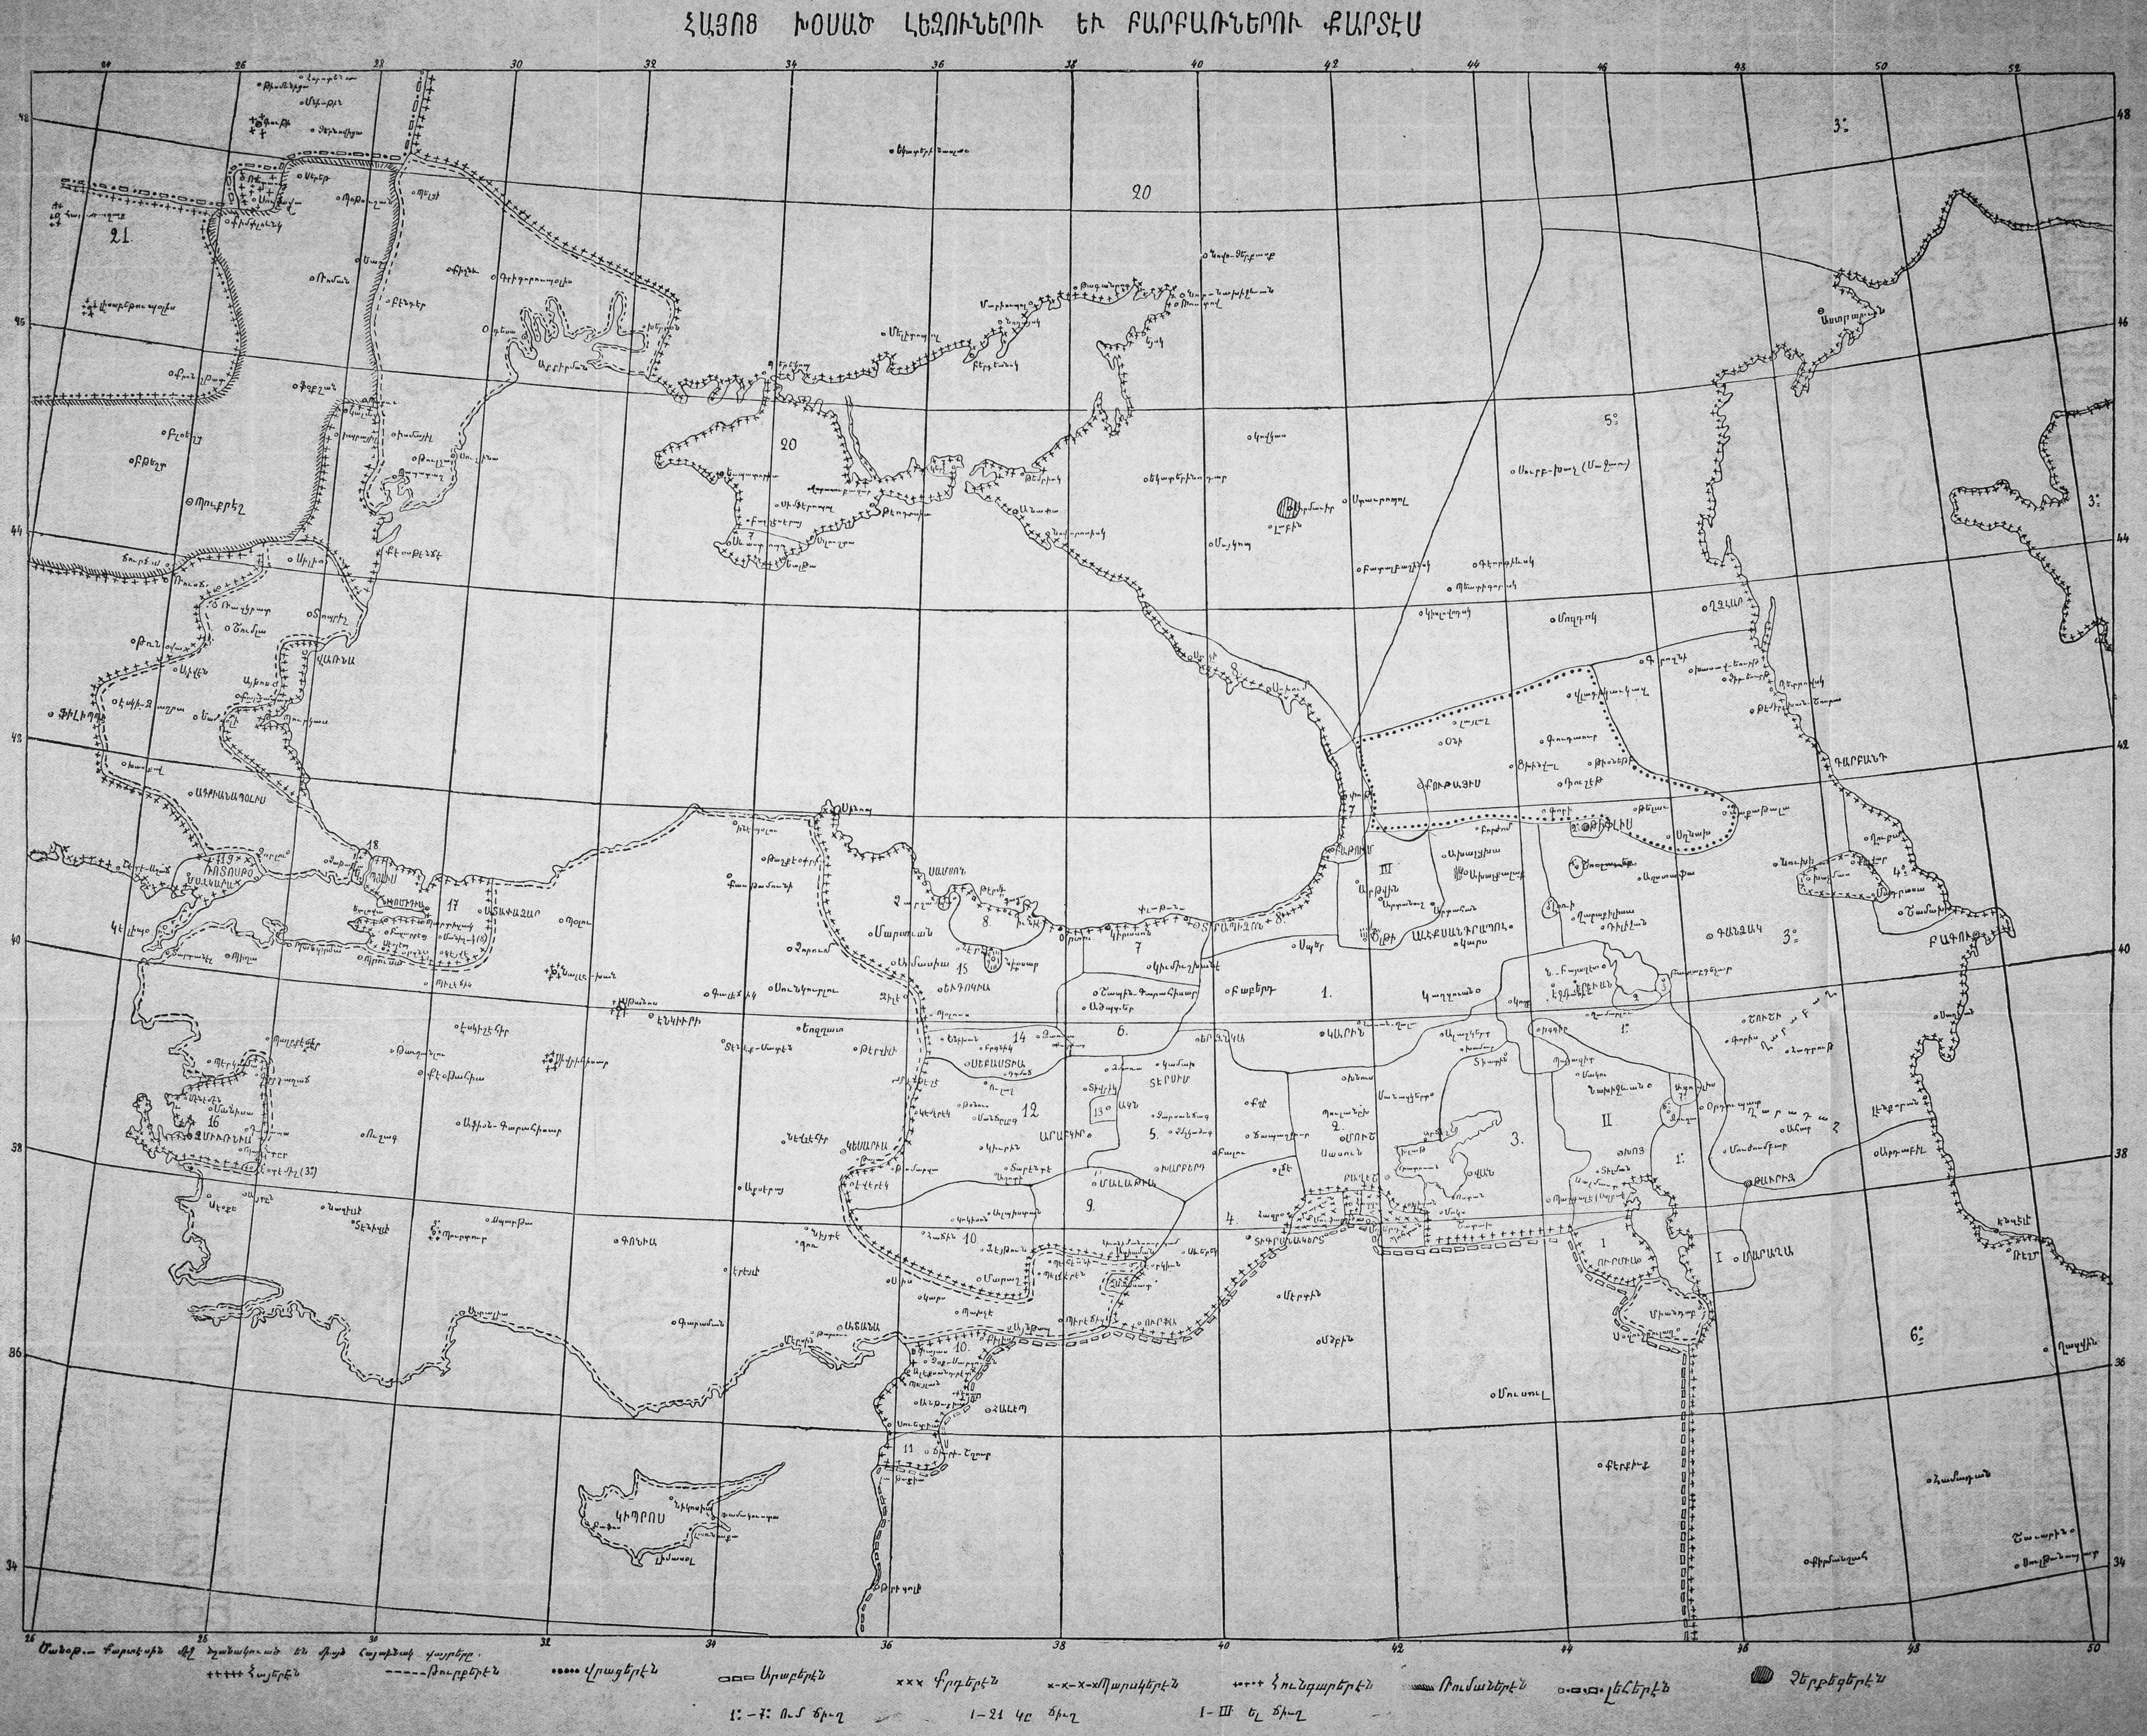
\includegraphics{images/map1911.png}
}
\end{figure}




In the original 1909 French monograph, Adjarian provided a similar map. It   is displayed in Figure \ref{map:Adjarian1909}. The names are all in Armenian. 

\begin{figure}[H]
	\caption{Map from Adjarian 1909}
	\label{map:Adjarian1909}
 \resizebox{\textwidth}{!}{%
	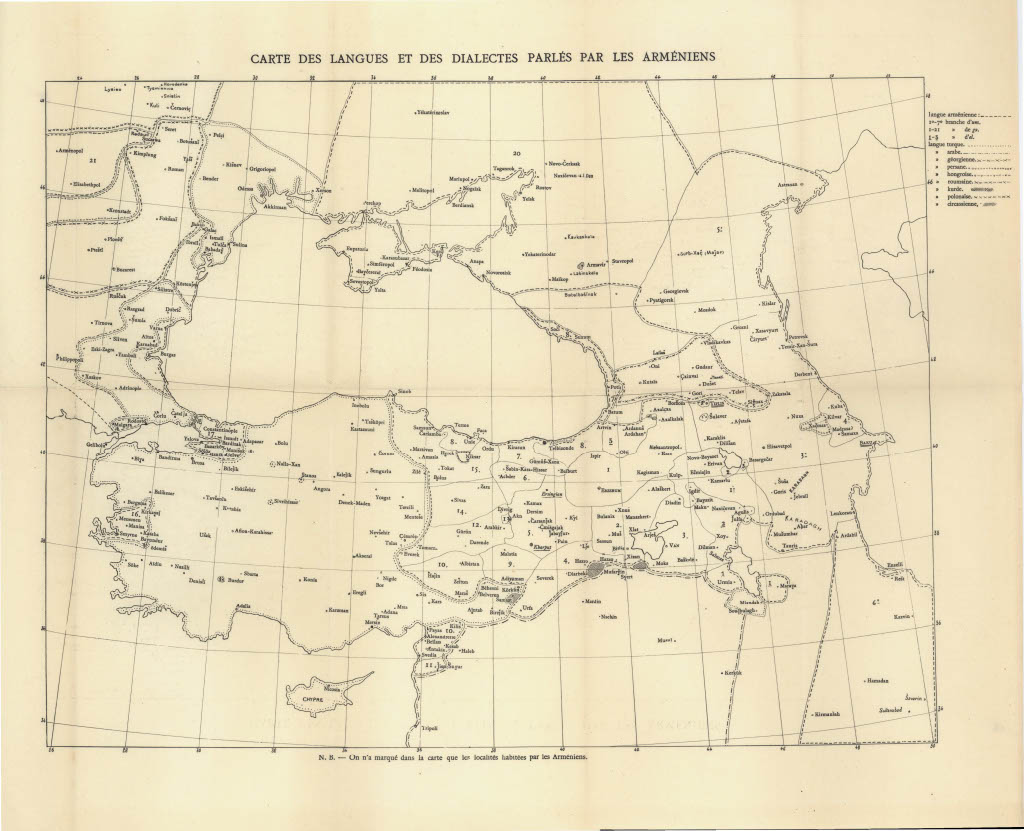
\includegraphics{images/map1909.jpg}
}
\end{figure}

On Wikimedia, a user had modified the 1909 map to add colorcoding to it.\footnote{\url{https://commons.wikimedia.org/wiki/File:Armenian_dialects,_Adjarian_1909.png}}.   is displayed in Figure \ref{map:Adjarian1909color}. The names are all in English; they don't however match the names that we used in our translation. 



\begin{figure}[H]
	\caption{Adapted map from Adjarian 1909 (from Wikimedia)}
	\label{map:Adjarian1909color}
	 \resizebox{\textwidth}{!}{%
		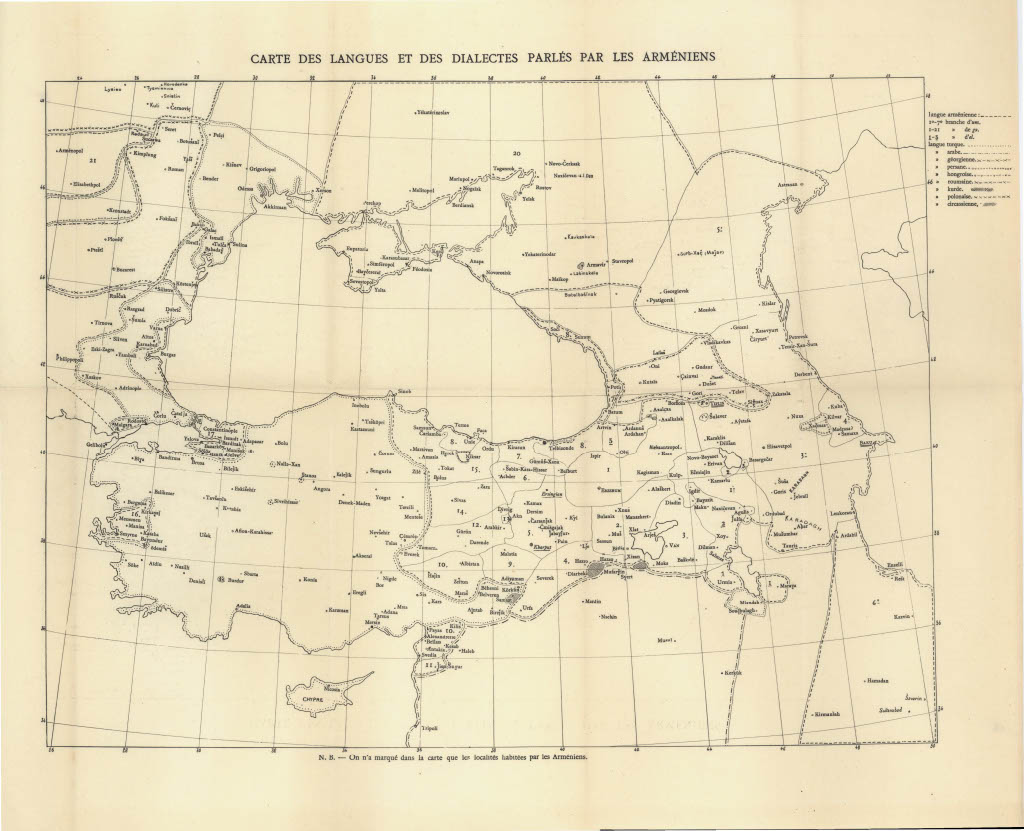
\includegraphics{images/map1909color.jpg}
}
\end{figure}
